\documentclass[crop, tikz, border=.1cm]{standalone}
\usetikzlibrary{positioning}
\usetikzlibrary{calc}
\usetikzlibrary{arrows.meta}
\begin{document}
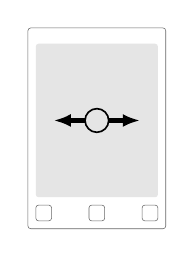
\begin{tikzpicture}[rounded corners=1, very thin]
    \newcommand\width{1.75}
\newcommand\height{2.55}
\newcommand\outborder{.1}
\newcommand\button{2 * \outborder}

\draw[black!60, fill=white] (0, 0) rectangle (\width, \height);

\fill[black!10]
    (\outborder, 4 * \outborder) coordinate (screen-bl) rectangle
    (\width - \outborder, \height - 2 * \outborder) coordinate (screen-tr);

\coordinate (screen-c) at ($(screen-bl)!.5!(screen-tr)$);

\draw[black!60] (\outborder, \outborder) rectangle
    ++(\button, \button);

\draw[black!60] (0.5 * \width - 0.5 * \button, \outborder) rectangle
    ++(\button, \button);

\draw[black!60] (\width - \outborder, \outborder) rectangle
    ++(-1 * \button, \button);

    \newcommand\radius{.15}

    \draw[semithick] (screen-c) circle (\radius);
    \draw[ultra thick, -{Latex[length=2.2mm]}]
        ($(screen-c)-(\radius,0)$) -- ++(-.4, 0);

    \draw[ultra thick, -{Latex[length=2.2mm]}]
        ($(screen-c)+(\radius,0)$) -- ++(.4, 0);
\end{tikzpicture}
\end{document}
